\documentclass[a4paper,oneside,11pt]{memoir}
\setsecnumdepth{subsection}

\usepackage[utf8]{inputenc} % input encoding
\usepackage[T1]{fontenc} % font encoding

\usepackage{graphicx} %to include images/graphics
\usepackage{amsmath,amssymb} %better math type setting
\usepackage{listings} %for source code snippets
\usepackage{textcomp} %for upquote
\usepackage{xcolor} % nice colors (for source code)
\usepackage{xltabular}
\usepackage[hidelinks]{hyperref}
\usepackage{awesomebox}
\usepackage{float}
\usepackage[verbose]{placeins} 

\renewcommand{\ttdefault}{pcr} % nicer font for source code

% an example configuration of the 'listings' package
\lstset{basicstyle=\ttfamily, 
        keywordstyle=\color{purple}\ttfamily,
        commentstyle=\color{gray}\ttfamily,
        stringstyle=\color{orange}\ttfamily,
        captionpos=b,
        float=tb,
        upquote=true,
}

\chapterstyle{tandh} % configuration of the 'memoir' class
\usepackage[backend=biber,style=ieee]{biblatex} % Use biblatex with the IEEE style
\addbibresource{mybibliography.bib} % Add your .bib file

%
% The actual document starts here
%
\begin{document}

\begin{titlingpage}
  \thispagestyle{empty}

  \centering
  \vspace*{6.5em}

  \textsc{\textbf{\huge
      % 
      % Insert your title here
      %
      Pokemon Battle Bot
    }}

  \vspace{4.5em}

  \textsc{
    \Large
    \textbf{Participants}
    \\[.4\onelineskip]
    \setlength{\tabcolsep}{12pt}
    \begin{tabular}[h]{lr}
      % 
      % Insert your names and exam numbers here
      %
      Anders Uttenthal Thomsen & 123456789
      \\[.4\onelineskip]
      Joachim Herborg Hviid    & 190402549
    \end{tabular}
  }

  \vspace{2em}

  \textsc{
    \Large
    \textbf{Supervisors\\}
    Parisa Niloofar
    \\[.4\onelineskip]
    Kamrul Islam Shahin
  }

  \vspace{5em}
  \large
  % 
  % Adjust the type of thesis and education here
  % 
  % Bachelor Project in Software Technology
  Bachelor Project in Software Engineering
  % Masters Project in Software Engineering

  \normalsize
  \vspace{2em}
  %
  % Change the date here
  %
  June 2025


  \vspace{12.5em}
  
\includegraphics[width=.5\textwidth]{assets/sdu_logo}

  \vspace{3em}
  The Maersk Mc-Kinney Moeller Institute

  \medskip
  University of Southern Denmark

\end{titlingpage}

\pagecolor{white}

\cleardoublepage

\frontmatter

% abstract / resume
\begin{abstract}
  Pokemon battles represent a complex and high-variance environment that is influenced by a wide range of mechanics such as 
  type advantages, status effects and stochastic events like move accuracy and critical hits. This project 
  investigates whether reinforcement learning can be used to optimize strategies within such an environment, and 
  whether knowledge gained from a trained agent can help human players improve their decision-making in Pokemon battles. 
  The study uses Deep Q-Networks (DQN) implemented with PyTorch and Gymnasium to train agents capable of playing Pokemon 
  battles. A custom battle simulator was developed to overcome the limitations of third-party environments and to provide 
  a fully controllable and extensible environment. The report details the design, implementation and iterative 
  development of both the agents and the environment, including handling of game mechanics, state representation 
  and reward functions. Evaluation includes agent performance over 10.000 self-play episodes 
  and profiling of the systems performance. The project concludes with reflections on learned agent behavior, performance 
  bottlenecks and opportunities for future improvement.
\end{abstract}


\cleardoublepage

\setcounter{tocdepth}{2}
\tableofcontents


\mainmatter

%
% We have one file per chapter:
%

\chapter{Introduction}
\label{chap:introduction}

    Pokemon is an old game that has continued to be relevant for nearly 30 years \cite{Pokemon}. 
During its lifespan there have been many different ways to enjoy the games, ranging from casually playing through them 
to competitive battles in international tournaments \cite{WaysToPlayPokemon}. Pokemon games have always had a lot of 
nuances in their gameplay, most notably battling. A Pokemon battle can have multiple formats, single, double or sometimes 
even triple battles. Different moves can have a chance of causing secondary effects. Attacks have a chance to critically 
strike the opponent causing significantly more damage than normal. These factors among others make Pokemon battles an 
interesting subject for analysis through AI agents \cite{PokeEnv}, as these effects can radically change the outcome 
of a battle. Training an agent to do well in a high variance environment like that can improve our general understanding 
of how to perform better in Pokemon battles.


\chapter{Requirements}
\label{chap:requirements}

hello


\chapter{Analysis and Design}
\label{chap:analysis-and-design}

\bigskip

\dots We summarize something in Table~\ref{tab:java-advantages}.

\begin{table}[tb] % placement: h for here, t for top, b for bottom
  \centering
  \begin{tabular}{l c}  % two columns: l for left, c for center, r for right
    Feature  & Benefit
    \\\hline
    Objects  & State encapsulation
    \\
    Generics & Code reuse
  \end{tabular}
  \caption{Advantages of Java}
  \label{tab:java-advantages}
\end{table}

\bigskip

\noindent
LaTeX indents a new paragraph unless you specify \lstinline{\noindent}.

\bigskip

We can also refer to Figure~\ref{fig:firefox-js-console}.

\begin{figure}[tb] % placement: h for here, t for top, b for bottom
  \centering
  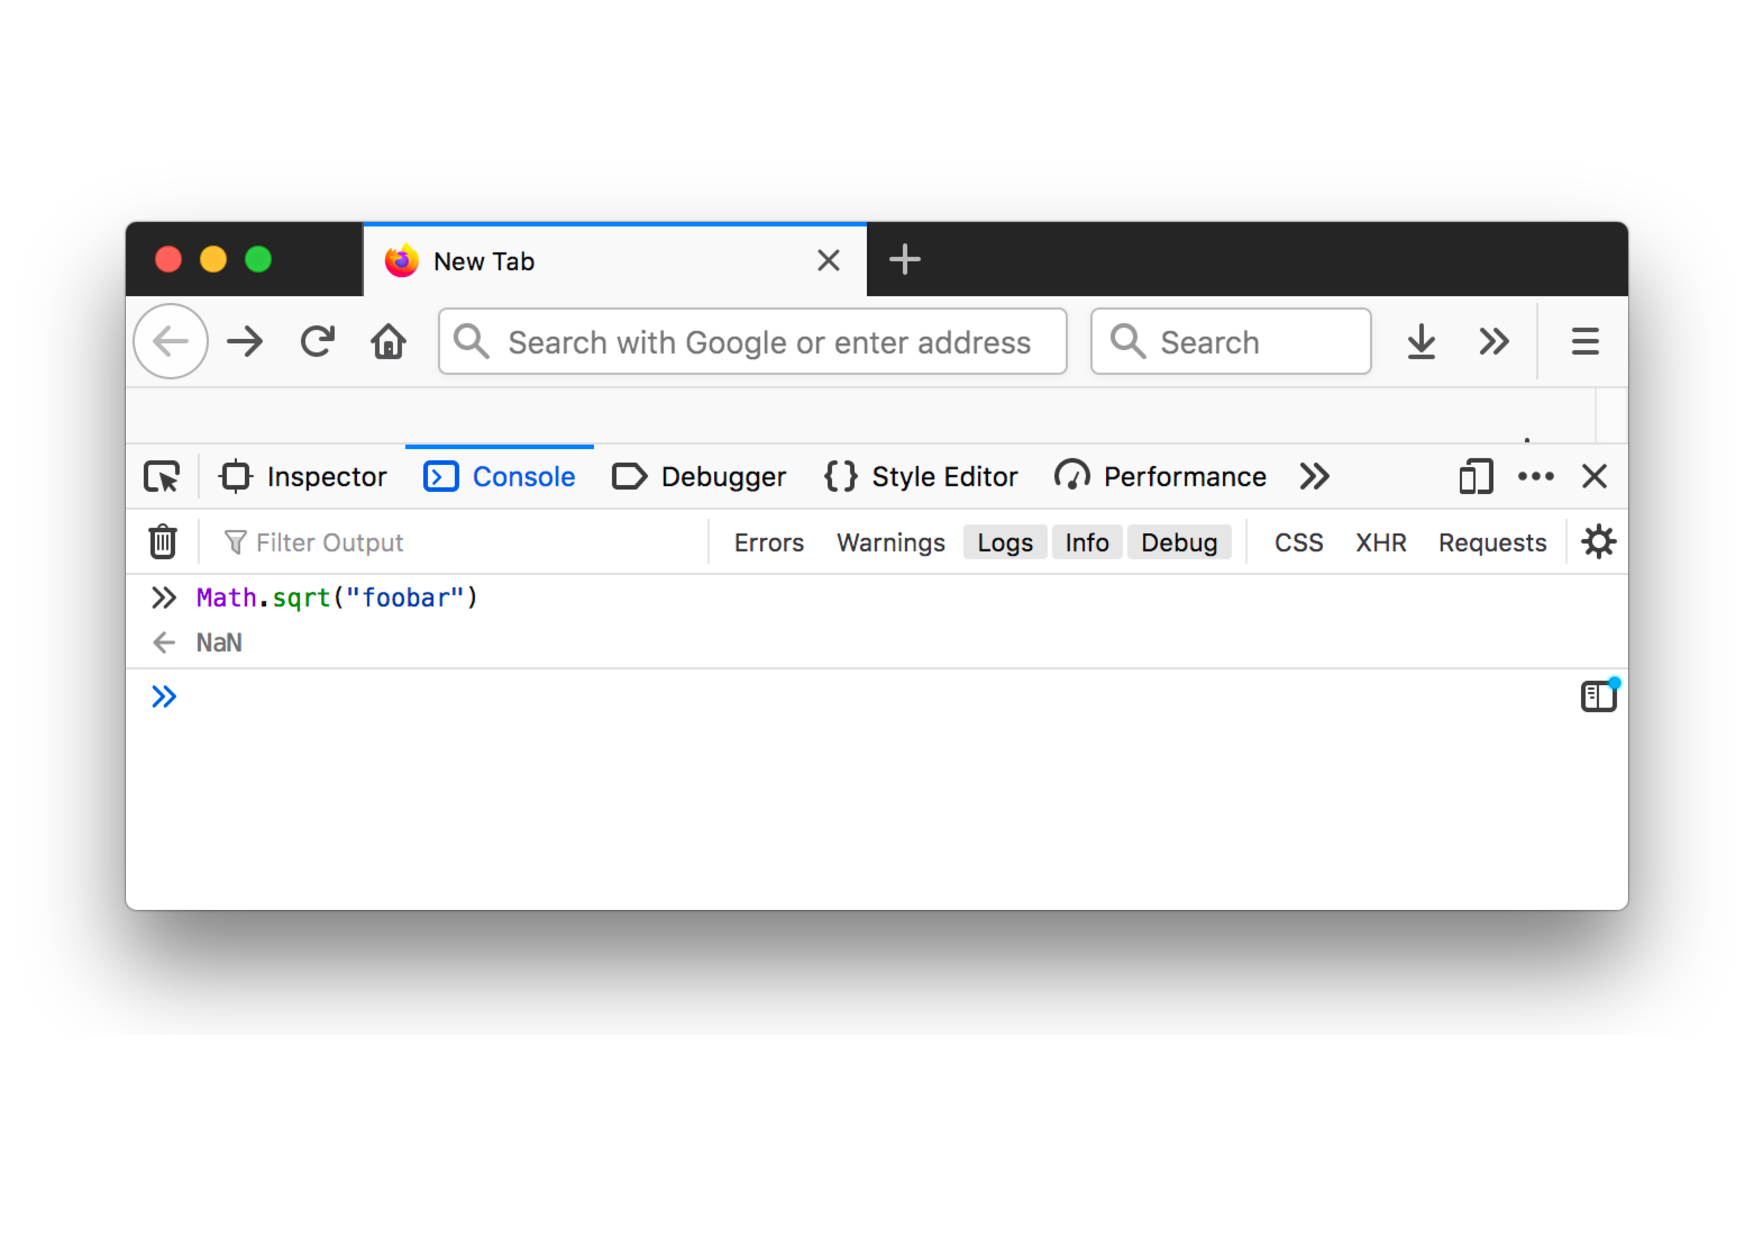
\includegraphics[width=.9\linewidth]{assets/firefox-js-console}
  \caption{The JavaScript console in Firefox }
  \label{fig:firefox-js-console}
\end{figure}


\chapter{Implementation}
\label{chap:implementation}

We can refer to Chapter~\ref{chap:analysis-and-design} for something.

\bigskip

Here is an example formula to compute a sum:
%
\begin{align*}
  \sum_{i=1}^{n} = \frac{n (n+1)}{2}
\end{align*}

Math can also be included inline $a (b + c) = a b + a c$ in a sentence.

\bigskip
We refer to Listing~\ref{lst:sum} for the Java implementation.\\ % force new line
Code snippets like \lstinline{System.out.println} can also be given inside a sentence.

\begin{lstlisting}[language=java,caption={Our sum implementation},float=tb,label=lst:sum]
  class Sum {
    public static void main(String[] args) {
      int n = 5;   // the input
      int sum = n * (n+1);
      System.out.println("The sum is: " + sum);
    }
  }
\end{lstlisting}

\bigskip

Finally we can refer to some material in Appendix~\ref{appendix:api-doc}. 


\chapter{Evaluation and Verification}
\label{chap:evaluation-and-verification}

% AI refinements?
\section{Process evaluation}
\label{sec:process-evaluation}

This project was made using agile principles and was split into 3 overall phases. Each phase corresponds to a section of
this report and had approximately 1 month of time allocated per phase. The phases were Project Planning 
(see chapters \ref{chap:introduction}, \ref{chap:requirements} and \ref{chap:analysis-and-design}), Development 
(see chapter \ref{chap:implementation}) and Evaluation and Conclusion (see chapters \ref{chap:evaluation-and-verification} 
and \ref{chap:conclusion}). At the end of each phase, the progress was presented to the supervisors in order to get some 
feedback and pointers for the work that needed to be focused on in the next phases. The goal of the phases were to mark 
important milestones in the project. Since the project was agile, the milestones did not prevent us from working on 
previous phase content, but they helped maintain focus on what was needed to be created at any given time.

The agile tools used by the project included, multiple weekly meetings discussing our progress, bi-weekly retrospective 
meetings and the use of Kanban boards to track tasks. The weekly meetings consisted of a mix of both online and in-person
meetings, to both discuss the project and do some collaboratory work like pair-programming or report writing. For more 
general communication, a Discord server was used. Here we also shared notes and sources we could use for the report and 
project.

Overall, these tools provided a strong foundation to our work process. Initially we had planned the phases to be 1 month
each, but as we progressed it became apparent that some phases needed more time than others. For instance, the
Development phase ended up taking closer to 1.5 months due to both technical difficulties during implementation, but also
due to assignments from different courses overlapping with the initial phase schedule.
The bi-weekly supervisor meetings and monthly presentations provided us with great feedback to work with in the initial
phases, but later in the process they were largely discontinued so that more time could be spent on building the project.
The weekly meetings with pair-programming also helped immensely early in the Development phase, but due to working different
aspects of the implementation these pair-programming sessions eventually evolved into debugging sessions, where we would
sit down and try to fix a technical problem together.
The Kanban board on Github helped maintain an overview of the tasks that needed to be done. It was split into Backlog, In Progress,
Review and Done. While the Kanban board was nice to have, we did not feel it provided too much value to the overall project.
This was likely due to the defined tasks being too broad or vague to definitively say whether a task was finished or not.
As a result, some tasks were accompanied by comments showing a long checklist of subtasks needed to complete the task. 
To borrow some terminology from SCRUM, some of the stories were in fact epics in disguise.

\section{Discussion}
\label{sec:discussion}

To round out this chapter, we will discuss the outcomes of this project. We will look back at what has been done
and reflect on how it compares with the initial problem statement. Then we will reflect on what we would do if we had more time.

\subsection{Did we solve the initial problem?}
Looking back to the problem described in section \ref{sec:problem-description}, it is stated that: 
\begin{quote}
  \itshape{We want to find out if it's possible to improve as a human player by analysing how a trained agent plays.}
\end{quote}
We created a custom environment and agent that was succesfully trained across thousands of episodes. After each training 
loop the agent became better and better. At the agents current level, it is unlikely to consistently beat a human opponent,
but given enough time and training, this agent will eventually become a stronger player, that we as humans can learn from.
Therefore, that part of the problem is considered solved.

An additional problem was described as:
\begin{quote}
  \itshape{We want to find out if it is possible to calculate the odds of winning a battle ahead of time given a predefined set of Pokemon.}
\end{quote}
This part was not fully implemented, but all of the necessary groundwork was created. The remaining work involved in solving
this part of the problem would be creating a command line interface where two files with team data could be specified. 
Then, the pre-trained AI model would be used to run 1.000-10.000 episodes depending on the desired accuracy. The amount of wins
and losses experienced during the episodes would then be returned to the user, who is then able to use this info to determine 
the odds of winning a given matchup. Additionally, a sample log could then be used to recreate the winning episodes.

\subsection{What would we do in the future?}
A lot of time was put into the creating of this project, however there is always room for improvements. If this project was to
be expanded upon, the first improvement would simply be to implement more mechanics. Going into this project, it was clear
that there would not be enough time to implement every single move, ability, held item and mechanics to the environment. 
For that reason, these mechanics were either completely omitted or only partially implemented in the current iteration, but
given more time, they must be fully implemented. During the implementation of the custom environment it dawned on us, just 
how much work there was in adding some of these mechanics, so this endeavour would also require a major refactoring in how
data is handled. This refactor would possibly look similar to how Pokemon Showdown \cite{PokemonShowdownSource} handles 
metadata of moves and abilities, by having multiple flags and events to listen to and extend.

Another thing that could be added with more time would be a graphical user interface (GUI). This would greatly increase useability for the users that
do not know how to use the command line. The GUI could also include a builtin team builder instead of relying on a file input.
In the far future, the GUI could be used as an overlay for the games to provide the user with move suggestions directly in the
client.

\section{The good and the bad parts}
\label{sec:good-bad-parts}

\subsection{Good parts}
The simulator works both with custom and external environments, providing great flexibility depending
on what kind of training is desired. The custom environment, while not fully feature complete, is open to extension and
can support multiple game environments, such as different generations of game rules. The external environment, Poke-env, 
supports most features found in the Pokemon games and comes with a visual replay option for presenting discovered strategies.

\subsection{Bad parts}
The custom environment is not feature complete. The simulator will only provide good results if its environment reflects
reality. While the missing features were declared in the initial requirements as optional for the purposes finishing the
project within the allotted time, they are crucial to provide accurate results to be used in a real product.

The training process is slower than anticipated. During training, we measured an average of 20 episodes per second. This 
is due to both environments being heavily CPU bound with limited processing able to be sent to the GPU. The training time
can most likely be improved in the custom environment by vectorizing the observations provided and by implementing 
multi-threading to divy up the work performed by the CPU to multiple threads. 



\chapter{Conclusion}
\label{chap:conclusion}

This project set out to explore whether reinforcement learning could be effectively applied to the complex and highly variable
environment of Pokemon battles. Through the development of a Deep Q-Network (DQN) agent and the construction of a custom
battle simulator, we have demonstrated that it is indeed possible to train an agent capable of engaging in
strategic decision-making within the Pokemon domain.

The project progressed through multiple iterations, starting with the use of 3rd party libraries like poke-env, and eventually
transitioning to a fully custom environment. This shift allowed for greater control over the simulation, improved performance
and the ability to tailor the environment specifically for reinforcement learning. A detailed implementation of game mechanics,
including various move effects, advanced battle logic and reward structures, enabled a vastly improved training process.

Training the agent through self-play over 10.000 episodes revealed positive learning trends and demonstrated the emergence of
informed behavior. Although reward parameters were sparse and the environment complexity posed various challenges, the agent displayed
signs of improvement and adaptation. Performance profiling further highlighted computational bottlenecks that then guided our future
optimization efforts.

The project also had a goal to provide a quick way to calculate the odds of a player winning a match given two teams of Pokemon.
The groundwork was done for this goal, but ultimately wasn't quite fleshed out enough to be usuable, due to a lack of userfacing
interface and API. 

Finally, this project validates the use of reinforcement learning for decision-making in turn-based, stochastic environments
like Pokemon battles. It also showcases the importance of simulation quality, effective reward design and iterative development 
processes when training AI agents. Future work could expand upon this foundation by introducing more advanced learning 
algorithms or integrating a GUI for analysis and human interactions.



\appendix

\chapter{Appendix}
\label{appendix:api-doc}

\section{Pokemon Type Chart}
\label{appendix:type-chart}

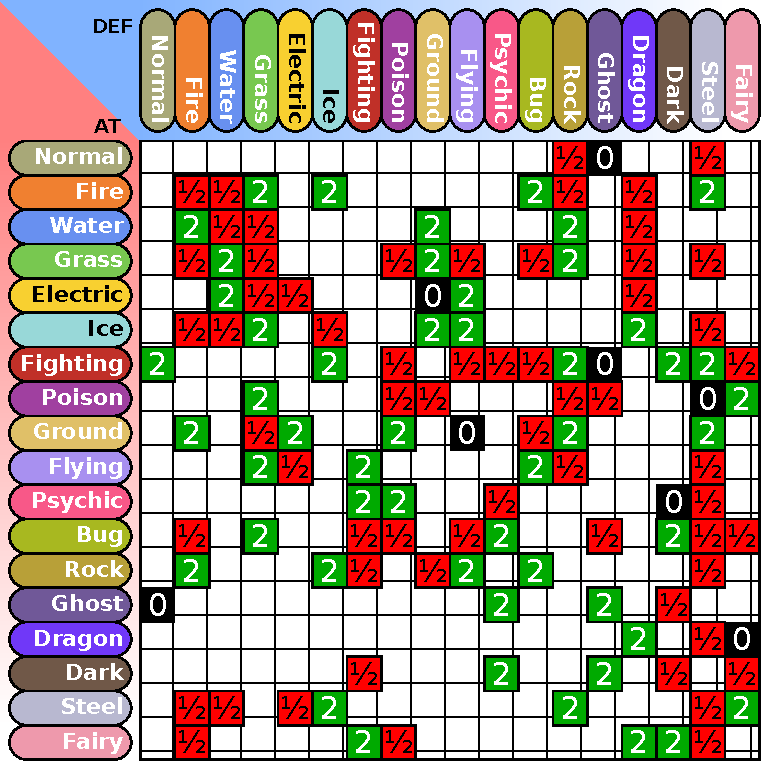
\includegraphics{assets/Pokemon_Type_Chart.pdf}
Image from bulbapedia \cite{TypeChart}

\clearpage
\section{Iteration graphs}
\label{appendix:iteration-graphs}

\begin{figure}[H]
    \includegraphics[width=.8\textwidth]{assets/Iteration-1-graphs.png}
    \caption{Iteration 1 - Baseline model trained over 1000 episodes}
    \label{fig:iteration-1-graphs}
\end{figure}

\begin{figure}[H]
    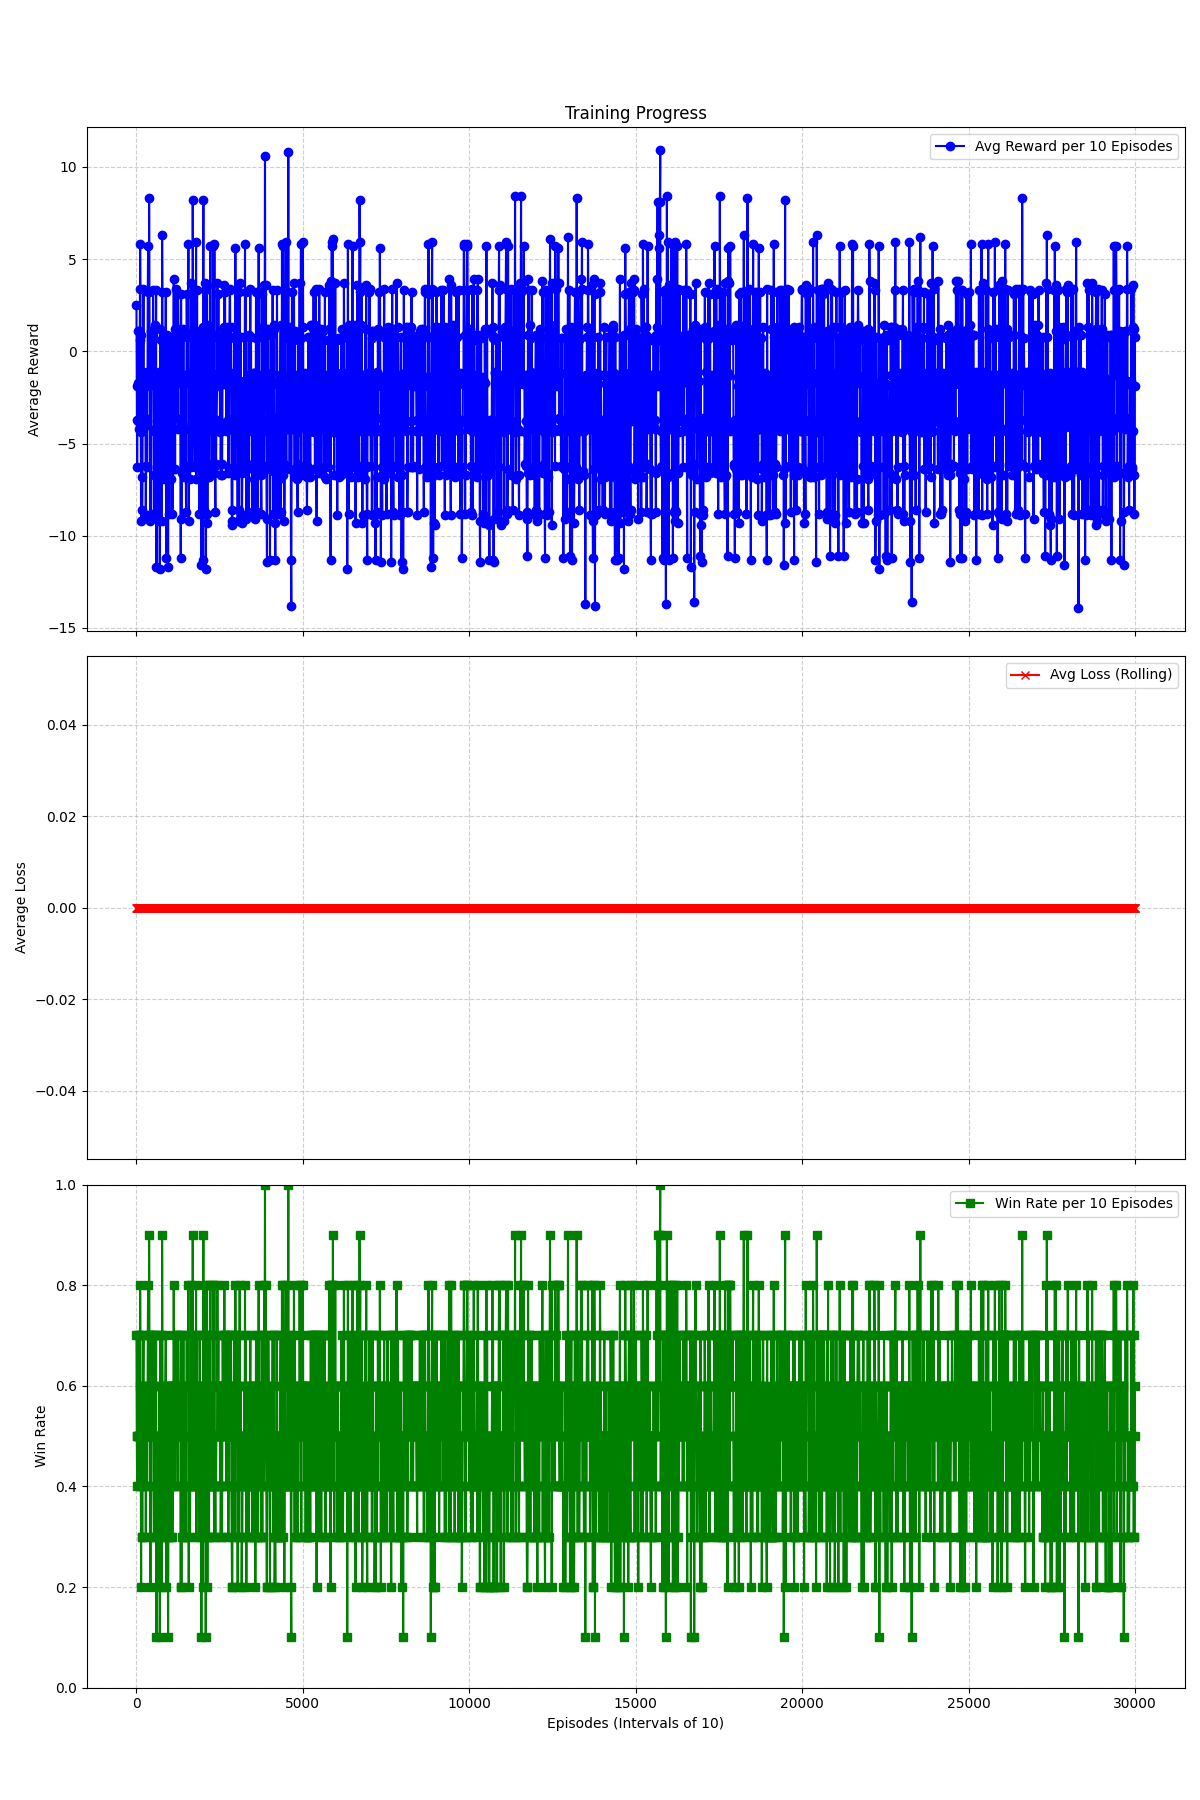
\includegraphics[width=.8\textwidth]{assets/Iteration-2-graphs.png}
    \caption{Iteration 2 - Enhanced model trained over 30000 episodes}
    \label{fig:iteration-2-graphs}
\end{figure}

\clearpage
\section{Poke-env cProfile}
\label{appendix:poke-env-cprofile}

\begin{changemargin}{-2cm}{-2cm}



\begin{lstlisting}[basicstyle=\fontsize{8}{8}\selectfont\ttfamily,language=Python,caption={Excerpt of Poke-env implementation cProfile sorted by time.}]
--- Script Execution Finished ---
         198618361 function calls (196480467 primitive calls) in 311.433 seconds

   Ordered by: internal time

   ncalls  tottime  percall  cumtime  percall filename:lineno(function)
        1  154.404  154.404  154.404  154.404 serialization.py:1141(_save)
271652/77   23.597    0.000    0.000    0.000 {built-in method _overlapped.GetQueuedCompletionStatus}
   189342   14.954    0.000   14.954    0.000 {built-in method torch.tensor}
    28097   13.472    0.000   13.472    0.000 {method 'run_backward' of 'torch._C._EngineBase' objects}
    28217    7.788    0.000   69.011    0.002 agentV2.py:244(learn)
   230844    6.869    0.000    6.869    0.000 {built-in method torch._C._nn.linear}
   386015    3.845    0.000    3.845    0.000 {method 'item' of 'torch._C.TensorBase' objects}
  3069996    3.339    0.000    9.412    0.000 target.py:35(from_showdown_message)
   324352    2.793    0.000    2.793    0.000 {built-in method numpy.array}
   180591    2.225    0.000   13.998    0.000 double_battle.py:256(get_possible_showdown_targets)
   338913    2.037    0.000    8.914    0.000 observed_pokemon.py:57(from_pokemon)
    88651    1.861    0.000    8.280    0.000 agentV2.py:332(embed_battle_doubles)
    25094    1.743    0.000    1.881    0.000 battle_order.py:82(join_orders)
  1025398    1.699    0.000    2.984    0.000 copy.py:248(_reconstruct)
   153896    1.658    0.000    1.658    0.000 {built-in method torch.relu}
  3075689    1.604    0.000    1.605    0.000 {method 'sub' of 're.Pattern' objects}
    28097    1.522    0.000    3.541    0.000 random.py:363(sample)
  1028322    1.493    0.000    5.667    0.000 copy.py:62(copy)
  3648050    1.104    0.000    1.708    0.000 random.py:245(_randbelow_with_getrandbits)
  3072778    1.053    0.000    3.743    0.000 __init__.py:183(sub)
   496872    1.020    0.000   11.872    0.000 abstract_battle.py:413(parse_message)
  1169228    1.012    0.000    1.629    0.000 double_battle.py:71(_get_active_pokemon)
7542218/7369342    0.961    0.000    1.222    0.000 {built-in method builtins.isinstance}
    48851    0.911    0.000    0.911    0.000 {method 'max' of 'torch._C.TensorBase' objects}
  9418982    0.889    0.000    0.889    0.000 {method 'replace' of 'str' objects}
  1242247    0.861    0.000    0.862    0.000 {method 'extend' of 'list' objects}
    28097    0.830    0.000    0.830    0.000 {built-in method torch._C._nn.smooth_l1_loss}
    28097    0.819    0.000    0.819    0.000 {built-in method torch._foreach_clamp_min_}
    30217    0.779    0.000  102.677    0.003 agentV2.py:467(choose_move)
    35600    0.742    0.000    0.742    0.000 {method 'WSASend' of '_overlapped.Overlapped' objects}
  4118786    0.730    0.000    0.730    0.000 {method 'split' of 'str' objects}
  3079682    0.729    0.000    1.151    0.000 __init__.py:330(_compile)
7730036/7699147    0.691    0.000    0.697    0.000 {built-in method builtins.len}
    28097    0.687    0.000    0.687    0.000 {method 'gather' of 'torch._C.TensorBase' objects}
  5970690    0.685    0.000    0.685    0.000 {method 'get' of 'dict' objects}
 144872/1    0.672    0.000    0.000    0.000 base_events.py:1953(_run_once)
    56194    0.662    0.000    0.662    0.000 {built-in method torch._ops.profiler._record_function_enter_new}
  3981553    0.648    0.000    0.982    0.000 enum.py:1308(__hash__)
    56194    0.604    0.000    0.604    0.000 {built-in method torch._foreach_add_}
    37072    0.601    0.000    2.041    0.000 double_battle.py:83(parse_request)
    28097    0.601    0.000    0.601    0.000 {built-in method torch._foreach_sqrt}
  1025398    0.585    0.000    0.585    0.000 {method '__reduce_ex__' of 'object' objects}
   106131    0.550    0.000  121.615    0.001 player.py:251(_handle_battle_message)
  8233225    0.544    0.000    0.545    0.000 {built-in method builtins.setattr}
    88651    0.527    0.000    2.398    0.000 _arraypad_impl.py:545(pad)
    76948    0.516    0.000   10.057    0.000 agentV2.py:171(forward)

\end{lstlisting}
\end{changemargin}
\clearpage
\section{Custom environment cProfile}
\label{appendix:custom-env-cprofile}

\begin{changemargin}{-2cm}{-2cm}

\begin{lstlisting}[basicstyle=\fontsize{8}{8}\selectfont\ttfamily,language=Python,caption={Excerpt of custom environment implementation cProfile sorted by time.}]
        45522147 function calls (44317837 primitive calls) in 72.082 seconds

  Ordered by: internal time

  ncalls  tottime  percall  cumtime  percall filename:lineno(function)
  25340    9.179    0.000    9.179    0.000 {method 'run_backward' of 'torch._C._EngineBase' objects}
  25460    7.725    0.000   47.040    0.002 battle_agent.py:99(train)
  223332    6.676    0.000    6.676    0.000 {built-in method torch._C._nn.linear}
  186428    3.844    0.000    3.845    0.000 {method 'to' of 'torch._C.TensorBase' objects}
  29672    2.942    0.000    9.161    0.000 battle_agent.py:62(choose_action)
  76020    1.989    0.000    1.989    0.000 {built-in method torch.cat}
  148888    1.778    0.000    1.778    0.000 {built-in method torch.relu}
  50680    1.575    0.000    1.575    0.000 {built-in method torch.stack}
  251568    1.044    0.000    2.084    0.000 pokemon.py:252(encode)
  29666    1.014    0.000    1.035    0.000 {built-in method _io.open}
  327844    0.940    0.000    0.940    0.000 {method 'item' of 'torch._C.TensorBase' objects}
  25340    0.806    0.000    0.806    0.000 {built-in method torch._C._nn.smooth_l1_loss}
  788606    0.727    0.000    0.729    0.000 {method 'extend' of 'list' objects}
  107732    0.696    0.000    0.696    0.000 {built-in method torch.tensor}
  25340    0.693    0.000    0.693    0.000 {method 'masked_fill' of 'torch._C.TensorBase' objects}
  25340    0.667    0.000    1.667    0.000 random.py:363(sample)
  31875    0.652    0.000    0.652    0.000 {method '__exit__' of '_io._IOBase' objects}
  25340    0.646    0.000    0.646    0.000 {built-in method torch._foreach_clamp_min_}
  27460    0.586    0.000    4.651    0.000 battle_agent.py:88(store_transition)
  25340    0.561    0.000    0.561    0.000 {built-in method torch._foreach_sqrt}
1697427    0.548    0.000    0.845    0.000 random.py:245(_randbelow_with_getrandbits)
  50680    0.539    0.000    0.539    0.000 {built-in method torch._ops.profiler._record_function_enter_new}
  50680    0.524    0.000    0.524    0.000 {built-in method torch._foreach_add_}
  74444    0.500    0.000   10.057    0.000 dqn.py:14(forward)
  25340    0.498    0.000    0.498    0.000 {built-in method torch.zeros}
  25340    0.481    0.000    0.481    0.000 {method 'gather' of 'torch._C.TensorBase' objects}
  25340    0.468    0.000    4.406    0.000 adam.py:534(_multi_tensor_adam)
  25340    0.448    0.000    0.448    0.000 {built-in method torch._foreach_addcdiv_}
  314496    0.448    0.000    0.448    0.000 _methods.py:99(_clip)
  268525    0.441    0.000    0.441    0.000 {built-in method numpy.array}
  25340    0.439    0.000    0.439    0.000 {method 'max' of 'torch._C.TensorBase' objects}
  78686    0.432    0.000    1.910    0.000 battle_agent.py:52(_flatten_observation)
  25340    0.414    0.000    0.414    0.000 {method 'any' of 'torch._C.TensorBase' objects}
  23764    0.405    0.000    0.405    0.000 {method 'clone' of 'torch._C.TensorBase' objects}
  25340    0.400    0.000    0.400    0.000 {built-in method torch.ones_like}
  25340    0.400    0.000    0.400    0.000 {built-in method torch._foreach_lerp_}
  25340    0.389    0.000    0.389    0.000 {built-in method torch._foreach_addcmul_}
  23764    0.382    0.000    0.382    0.000 {method 'argmax' of 'torch._C.TensorBase' objects}
297776/74444    0.381    0.000   10.298    0.000 module.py:1755(_call_impl)
  62892    0.315    0.000    0.366    0.000 shape_base.py:380(stack)
  786860    0.311    0.000    0.311    0.000 {method 'flatten' of 'numpy.ndarray' objects}
  214698    0.304    0.000    0.304    0.000 {method 'reduce' of 'numpy.ufunc' objects}
  50680    0.303    0.000    0.303    0.000 {built-in method torch._C._group_tensors_by_device_and_dtype}
  25340    0.302    0.000    0.472    0.000 adam.py:137(_init_group)
      1    0.295    0.295    0.390    0.390 __init__.py:158(_load_dll_libraries)
297776/74444    0.288    0.000   10.388    0.000 module.py:1747(_wrapped_call_impl)
  74444    0.286    0.000    0.286    0.000 {method 'unsqueeze' of 'torch._C.TensorBase' objects}
2773908/2597068    0.284    0.000    0.444    0.000 {built-in method builtins.isinstance}
  670068    0.269    0.000    0.269    0.000 module.py:1927(__getattr__)
  62892    0.264    0.000    2.207    0.000 battle_state.py:24(encode_team)
  25340    0.260    0.000    1.198    0.000 optimizer.py:931(zero_grad)
  88380    0.253    0.000    0.610    0.000 multi_binary.py:124(contains)


\end{lstlisting}
\end{changemargin}
\clearpage

\printbibliography

\end{document}
